% Preden se lotite pisat, preberite navodila v "editor.tex"
% Zapiski:
% - vse labele se morejo zacet z "g19:"
% - slike grej v Skupina19/img
% - vse slike so v .pdf/.eps formatu
% - vse reference grejo v references.bib

\graphicspath{{Skupina19/img/}}


\title{Enodimenzionalni celularni avtomati v QCA}
\author{Enei Sluga, Matej Urbas, Lan Vukušič, Jan Vasiljević}

\institute{Enei Sluga \at FRI, UNI LJ, \email{es6878@studnet.uni-lj.si}
    \and  Matej Urbas \at FRI, UNI LJ \email{mu6188@studnet.uni-lj.si}
    \and Lan Vukušič \at FRI, UNI LJ, \email{lv8541@studnet.uni-lj.si}
    \and Jan Vasiljević \at FRI, UNI LJ, \email{jv1721@student.uni-lj.si}
}


% Use the package "url.sty" to avoid
% problems with special characters
% used in your e-mail or web address
%
\maketitle


\abstract{
    V seminarski nalogi smo se ukvarjali z implementacijo enodimenzionalnega celičnega avtomata s tehnologijo kvantnih celičnih avtomatov.
    Zasnovali smo QCA vezje, ki temelji na 3-8 dekodirniku in pomožnih logičnih vratih.
    Na podlagi sorodnih del smo implementirali dva 3-8 dekodirnika in se nato zaradi bolj praktične fizične implementacije odločili za enega izmed njiju.
    S pomočjo majoritetnih vrat smo izdelali končno vezje, ki je sposobno izvajati enodimenzionalni celični avtomat s poljubnim 8-bitnim pravilom.
    Celotno vezje smo implementirali v orodju QCADesigner.}

\newpage
\section{Uvod}
\label{g19:sec:uvod}


Enodimenzionalni celični avtomat je matematični model, sestavljen iz vrste celic, kjer vsaka celica lahko prevzame eno od končnega števila stanj.
Stanje celice se spreminja v diskretnih časovnih korakih glede na preprosta pravila, odvisna od stanja sosednjih celic.
Ti avtomati ustvarjajo kompleksno obnašanje iz preprostih pravil.
V pomoč so pri raziskovanju kompleksnih sistemov in vzorcev ter se pogosto uporabljajo v študijah samoorganizacije, računalništva in teorije kompleksnosti.

\begin{figure}[H]
    \sidecaption
    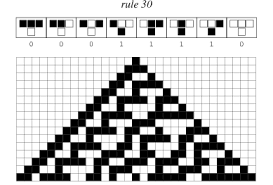
\includegraphics[width=0.6\textwidth]{1d-automata.png}
    \caption{Primer izhodov 1D celularnega avtomata. Vsaka vrsta predstavlja novo posodobitev stanja glede na pravilo \textit{30}.}
    \label{g19:fig:1d-automata}
\end{figure}

V naši nalogi se posvečamo elementarnim enodimenzionalnim celičnim avtomatom \ref{g19:fig:1d-automata}, kjer ima vsaka celica dve možni stanji, 0 ali 1.
Pravilo, ki določa naslednje stanje celice, je odvisno od trenutnega stanja celice in njenih dveh sosedov, kar pomeni, da je pravilo odvisno od treh bitov oziroma osmih možnih kombinacij.
Obstaja 256 različnih pravil, vsako pa je mogoče predstaviti z 8-bitno binarno številko, t. i. Wolframovim kodom.

Za implementacijo bomo uporabili kvantne celične avtomate (QCA), ki so alternativna tehnologija za izdelavo logičnih vezij.
QCA temelji na kvantnih lastnostih elektronov in njihovih interakcijah.
QCA vezja omogočajo nizko porabo energijee in visoko gostoto integracije.
Podobne implementacije, osredotočene na Conwayevo igro življenja, so že bile razvite \cite{conway}. V našem primeru se bomo osredotočili na preprostejše primere, ki zasedejo manj prostora pri fizični implementaciji.

\section{Metode}

Vezje avtomata smo sprva predstavili z logičnimi vrati. Osnovni koncept vezja je prikazan na Sliki \ref{g19:fig:koncept}.
Vezje ima tri vhode, ki predstavljajo trenutno stanje celice in njenih dveh sosedov, ter en izhod, ki predstavlja naslednje stanje sredinske celice.
Ima tudi 8 vhodnih vhodnih bitov, s katerimi določimo pravilo avtomata.

Najbolj pomemben del vezja je 3-8 dekodirnik, ki ugotovi, v katerem od osmih možnih stanj se nahaja sredinska celica.
Drugi del vezja preveri, če stanje celic ustreza pravilu in tako določi naslednje stanje sredinske celice.
Sestavljen je iz osmih AND vrat in sedmih OR vrat.
Vrata AND preverijo, če je trenutno stanje celice v pravilu, vrata OR pa združijo izhode AND vrat v končni izhod.


\begin{figure}[H]
    \sidecaption
    \includegraphics[width=1.0\textwidth]{vezje.pdf}
    \caption{Konceptualna zasnova vezja sestavljenega iz 3-8 dekodirnika, osmih AND vrat in sedmih OR vrat.}
    \label{g19:fig:koncept}
\end{figure}

Implementacija vezja je v celoti mogoča z uporabo majoritetnih vrat, ki lahko delujejo kot AND ali OR vrata, odvisno od vhodnih bitov.
V tehnologiji QCA so majoritetna vrata sestavljena iz petih celic, postavljenih v obliki znaka plus.
Tri zunanje celice delujejo kot vhod, četrta pa kot izhod vezja.
Če en vhodni bit nastavimo na 0, bodo majoritetna vrata na preostalih dveh vhodih delovala kot vrata AND, sicer pa kot vrata OR.

\begin{table}
    \centering
    \begin{tabular}{|l|l|}
        \hline
        \textbf{Element} & \textbf{Število elementov} \\ \hline
        AND vrata        & 8                          \\ \hline
        OR vrata         & 7                          \\ \hline
        3-8 dekodirnik   & 1                          \\ \hline
    \end{tabular}
    \caption{Tabela števila elementov uporabljenih pri realizaciji klasičnega vezja.}
\end{table}

\subsection{Implementacija dekodirnika}

Za implementacijo 3-8 dekodirnika smo sprva pregledali že obstoječe rešitve \cite{3_8decoder_1, 3_8decoder_2}.
Izbirali smo med dvema implementacijama, ki se razlikujeta v fizični postavitvi celic.
Obe implementaciji sta sestavljeni iz dvanajstih majoritetnih vrat in treh slojev, od katerih je en povezovalni.
Prav tako obe implementaciji za obdelavo potrebujeta tri četrtine urinega cikla.

Sprva smo implementirali dekodirnik iz \cite{3_8decoder_2}.
Realizacija v QCADesigner-ju pa je vidna na Sliki \ref{g19:fig:enc1}.
S simulacijo smo tudi potrdili njegovo pravilno delovanje (Slika \ref{g19:fig:enc1_graph}).
Implementacija je zelo kompaktna, saj jo je mogoče realizirati na površini 11x24 QCA celic in treh slojih.
Največja slabost te implementacije je, da so izhodi postavljeni v sredini vezja, direktno nad spodnjim slojem, kar otežuje povezavo z ostalimi elementi našega končnega avtomata.
Če bi v končnem avtomatu uporabili ta dekodirnik, bi moralo biti končno vezje sestavljeno iz petih slojev, kar bi povečalo kompleksnost in možnost napak.

Implementirali smo tudi dekodirnik iz \cite{3_8decoder_1} ter ga nekoliko prilagodili.
Prilagojeno vezje je prikazano na Sliki \ref{g19:fig:enc2}.
Vezje se od originala razlikuje v vodilu vhoda A, ki se preostalemu vezju priključi na sredini.
S tem smo odpravili napako, ki se pojavi zaradi pojemajočega signala.
Prav tako smo zamenjali obliko vrat NOT in tako porabili manj celic.
To vezje je prav tako sestavljeno iz dvanajstih majoritetnih vrat in treh slojev, vendar se izhodi nahajajo na bolj obrobnih mestih, kar poenostavi njihovo uporabo v končnem vezju.
Celotno vezje je sicer večje od prejšnjega in zavzema površino 20x32 QCA celic, vendar je zaradi bolj razpršene postavitve celic lažje povezljivo z ostalimi elementi avtomata.
Z uporabo te implementacije 3-8 dekodirnika smo lahko končno vezje v celoti realizirali na treh slojih.

Pri drugem dekodirniku smo tudi opazili zelo specifične vrednosti polarizacije fiksnih celic, ki so bile potrebne za pravilno delovanje majoritetnih vrat.
Ker se nam je zdelo, da take vrednosti polarizacije ni mogoče doseči v praksi, smo se odločili, da vrednosti polarizacije nastavimo na -1.
Simulacija je nato delovala pravilno samo, če smo povečali število vzorcev bistabilne aproksimacije na 100 000.

\begin{figure}[H]
    \sidecaption
    \includegraphics[width=1.0\textwidth]{enc1.pdf}
    \caption{Prvi testiran 3-8 dekodirnik. Na levi strani je prikazan spodnji nivo vezja, na desni pa zgornji. Povezovalni nivo ni prikazan.}
    \label{g19:fig:enc1}
\end{figure}

\begin{figure}[t]
    \sidecaption
    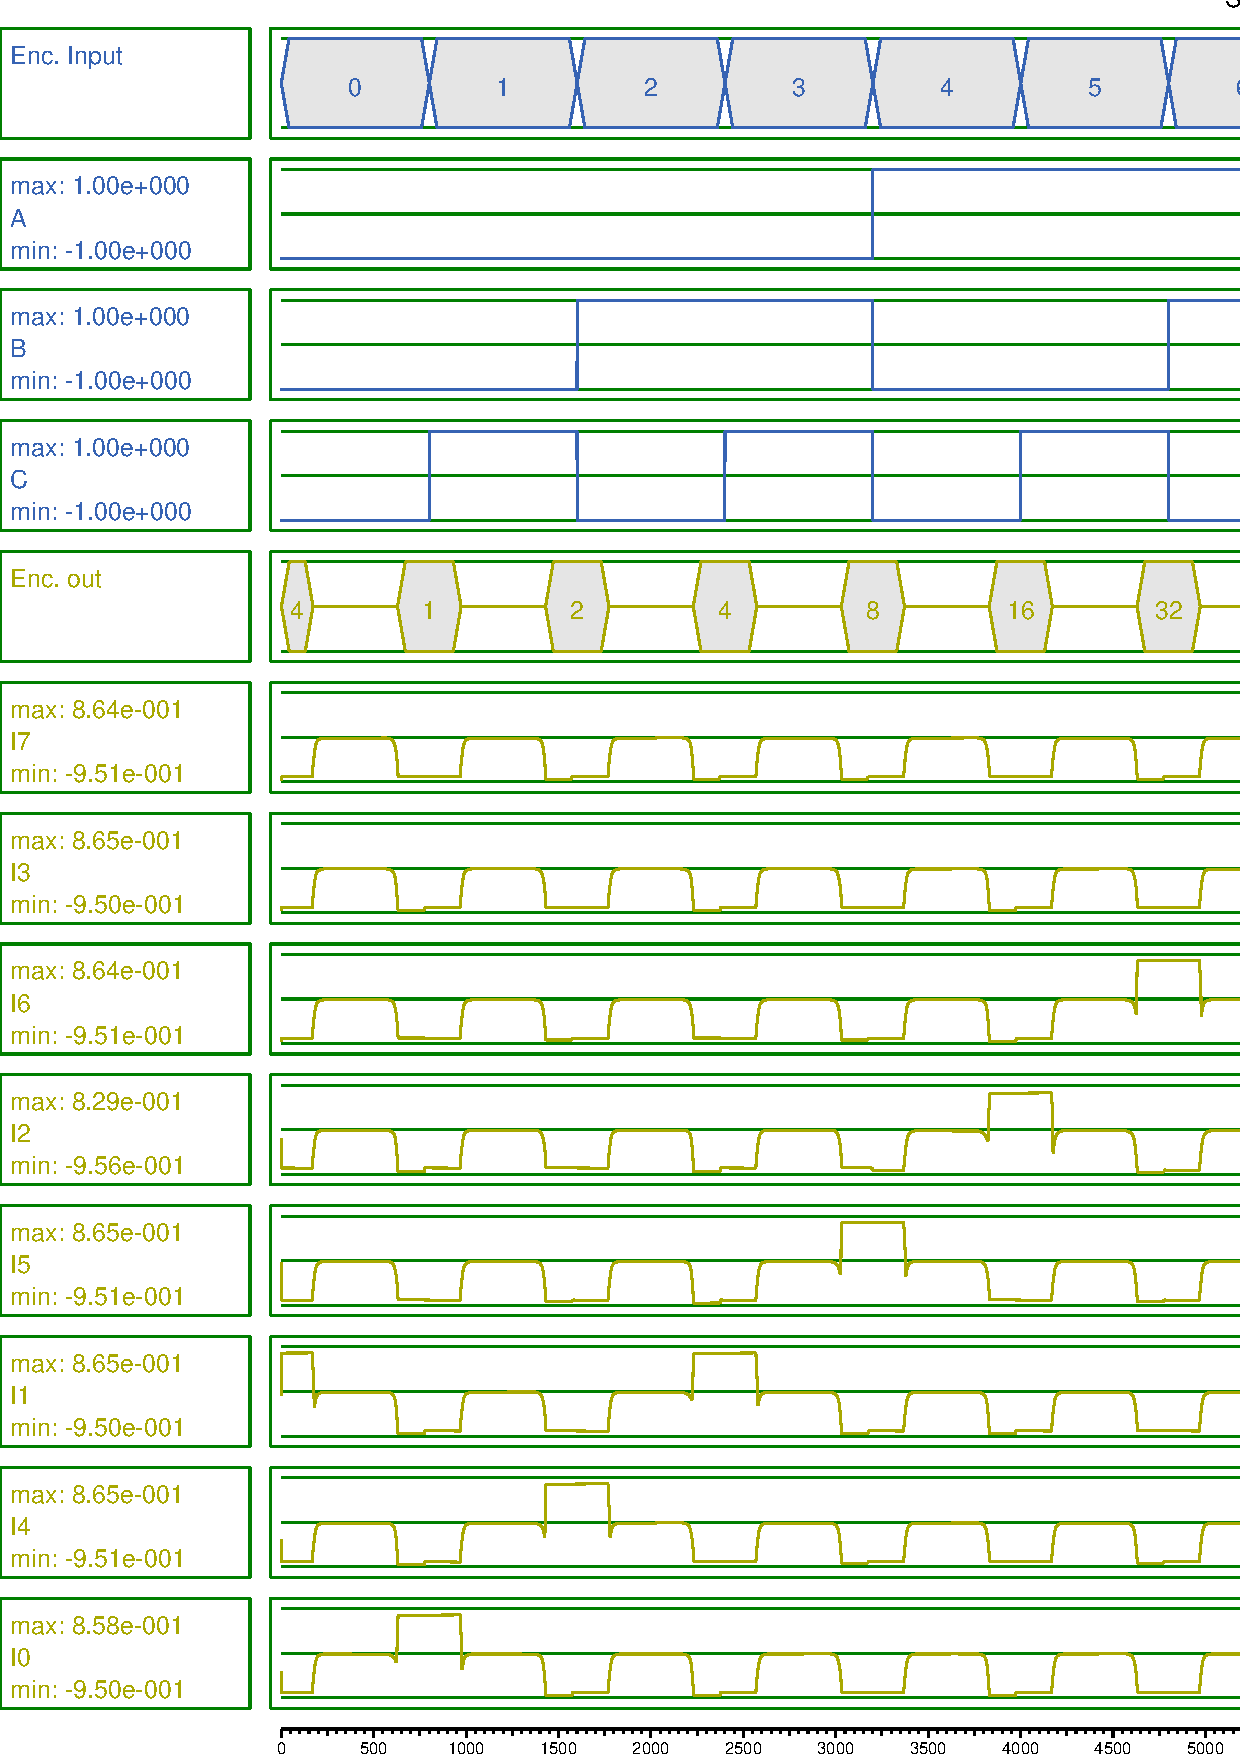
\includegraphics[width=1.0\textwidth]{encoder_graph}
    \caption{Označeni vhodi (A,B,C) in izhodi (I od 0-7) dekodirnika. Celice so povezane v vodila \textit{bus} in pretvorjena v decimalni sistem za lažjo interpretacijo.}
    \label{g19:fig:enc1_graph}
\end{figure}

\begin{figure}[H]
    \sidecaption
    \includegraphics[width=1.0\textwidth]{enc2.pdf}
    \caption{Drugi testiran 3-8 dekodirnik. Spodnji sloj vezja je v bolj osvetljeni barvi, zgornji pa v temnejši.}
    \label{g19:fig:enc2}
\end{figure}

\subsection{Implementacija izbire naslednjega stanja}
Implementacijo vezja za izbiro naslednjega stanja smo implementirali sami.
Desni del konceptualnega vezja iz Slike \ref{g19:fig:koncept} smo enostavno realizirali z uporabo petnajstih majoritetnih vrat.
Struktura vezja je prikazana na Sliki \ref{g19:fig:next_state}.

\begin{figure}[H]
    \sidecaption
    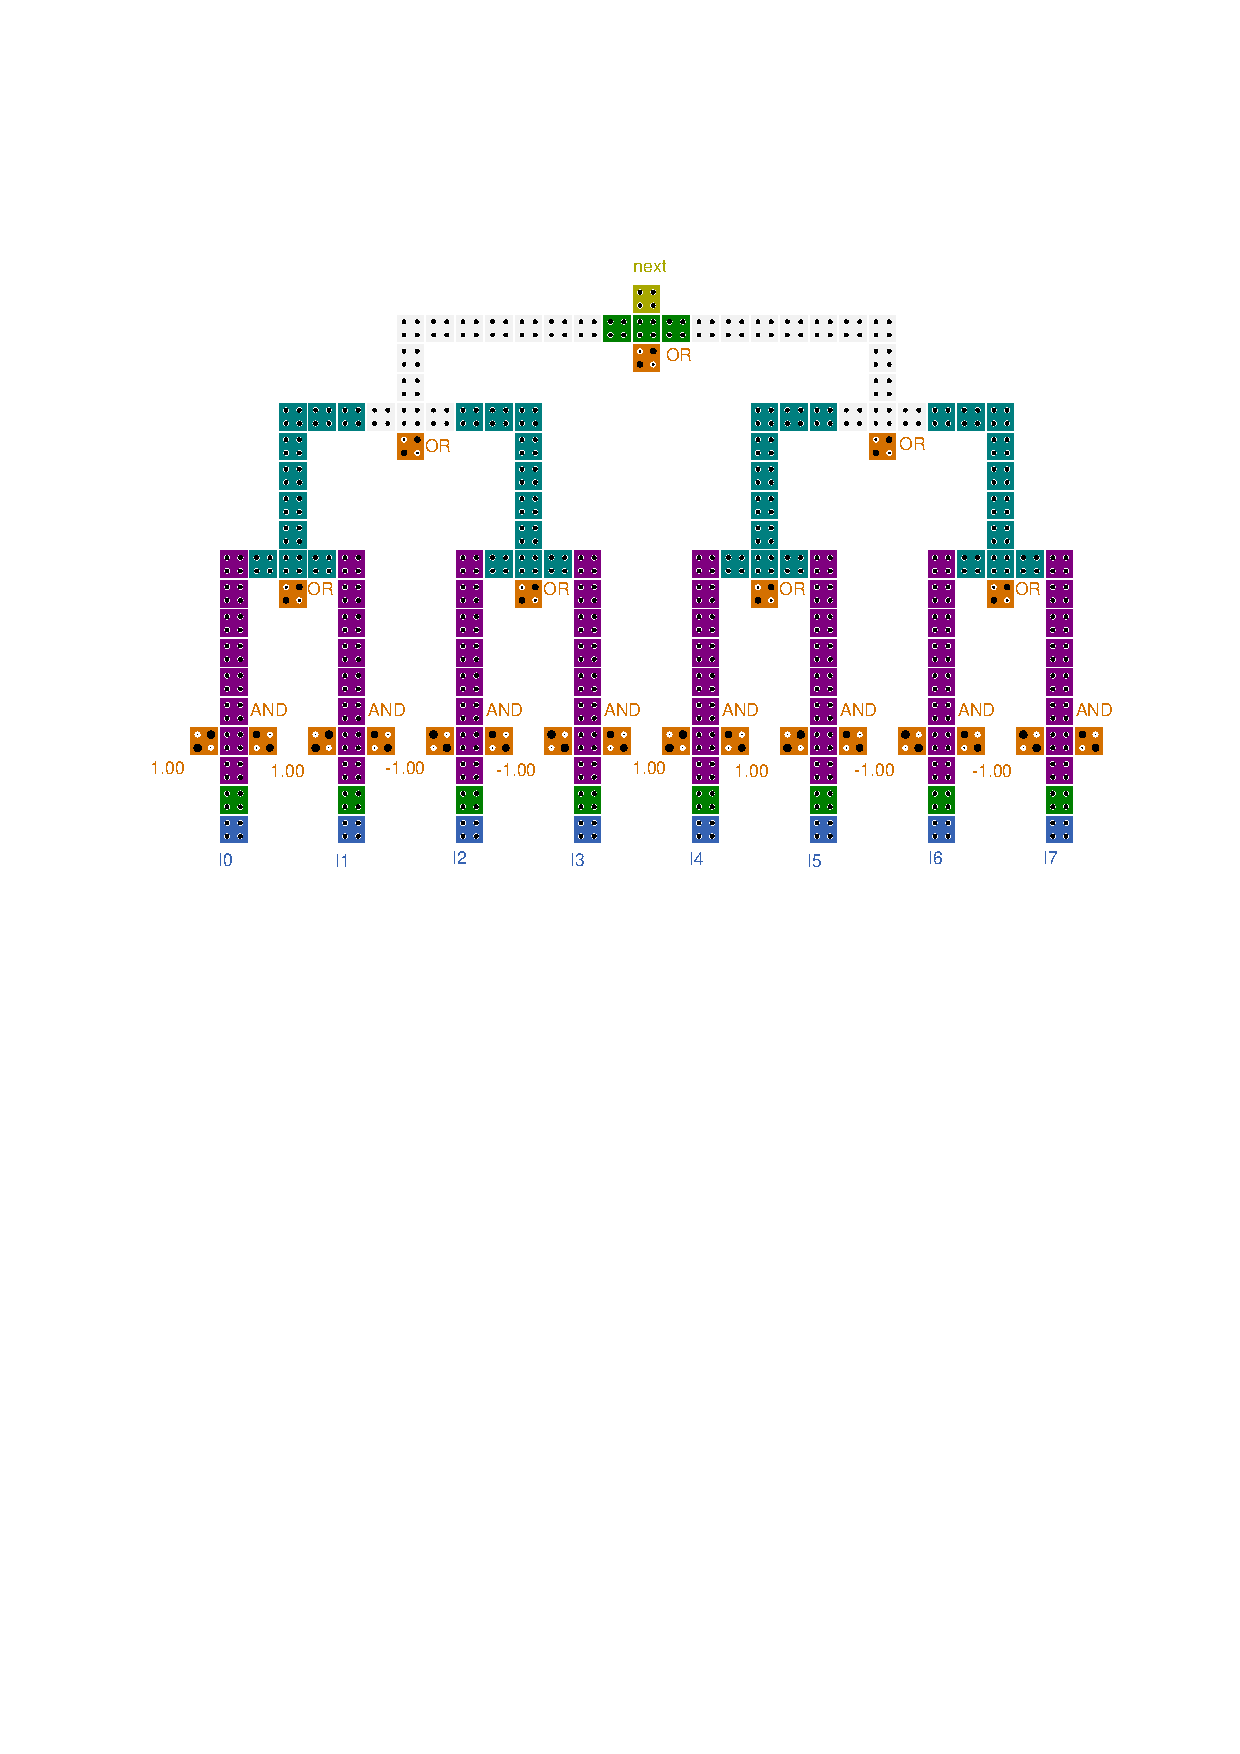
\includegraphics[width=1.0\textwidth]{next_state}
    \caption{Vezje za izbiro naslednjega stanja s pravilom 204.}
    \label{g19:fig:next_state}
\end{figure}

Struktura ima osem vhodov in en sam izhod. Vhodi v to strukturo bodo prihajali iz izhodov dekodirnika, izhod pa bo predstavljal naslednje stanje sredinske celice.
Vhodi so povezani na osem majoritetnih vrat, ki izvajajo funkcijo AND.
Poleg vhodov tukaj definiramo pravilo našega avtomata.
Na Sliki \ref{g19:fig:next_state} je prikazano pravilo \textit{204}, kar je razvidno iz vrednosti polarizacije fiksne celice na levi strani vsake od majoritetnih vrat (1, 1, -1, -1, 1, 1, -1, -1 predstavlja 0b11001100, kar je 204).

\subsection{Implementacija končnega vezja}
Končno vezje je sestavljeno iz izbranega 3-8 dekodirnika in vezja za izbiro naslednjega stanja.
Za prenos izhoda dekodirnika na vezje za izbiro naslednjega stanja smo vodilo enostavno premaknili na spodnji sloj, kjer smo postavili vezje za izbiro naslednjega stanja.
Končno vezje je prikazano na Sliki \ref{g19:fig:final}.

\begin{figure}[t]
    \sidecaption
    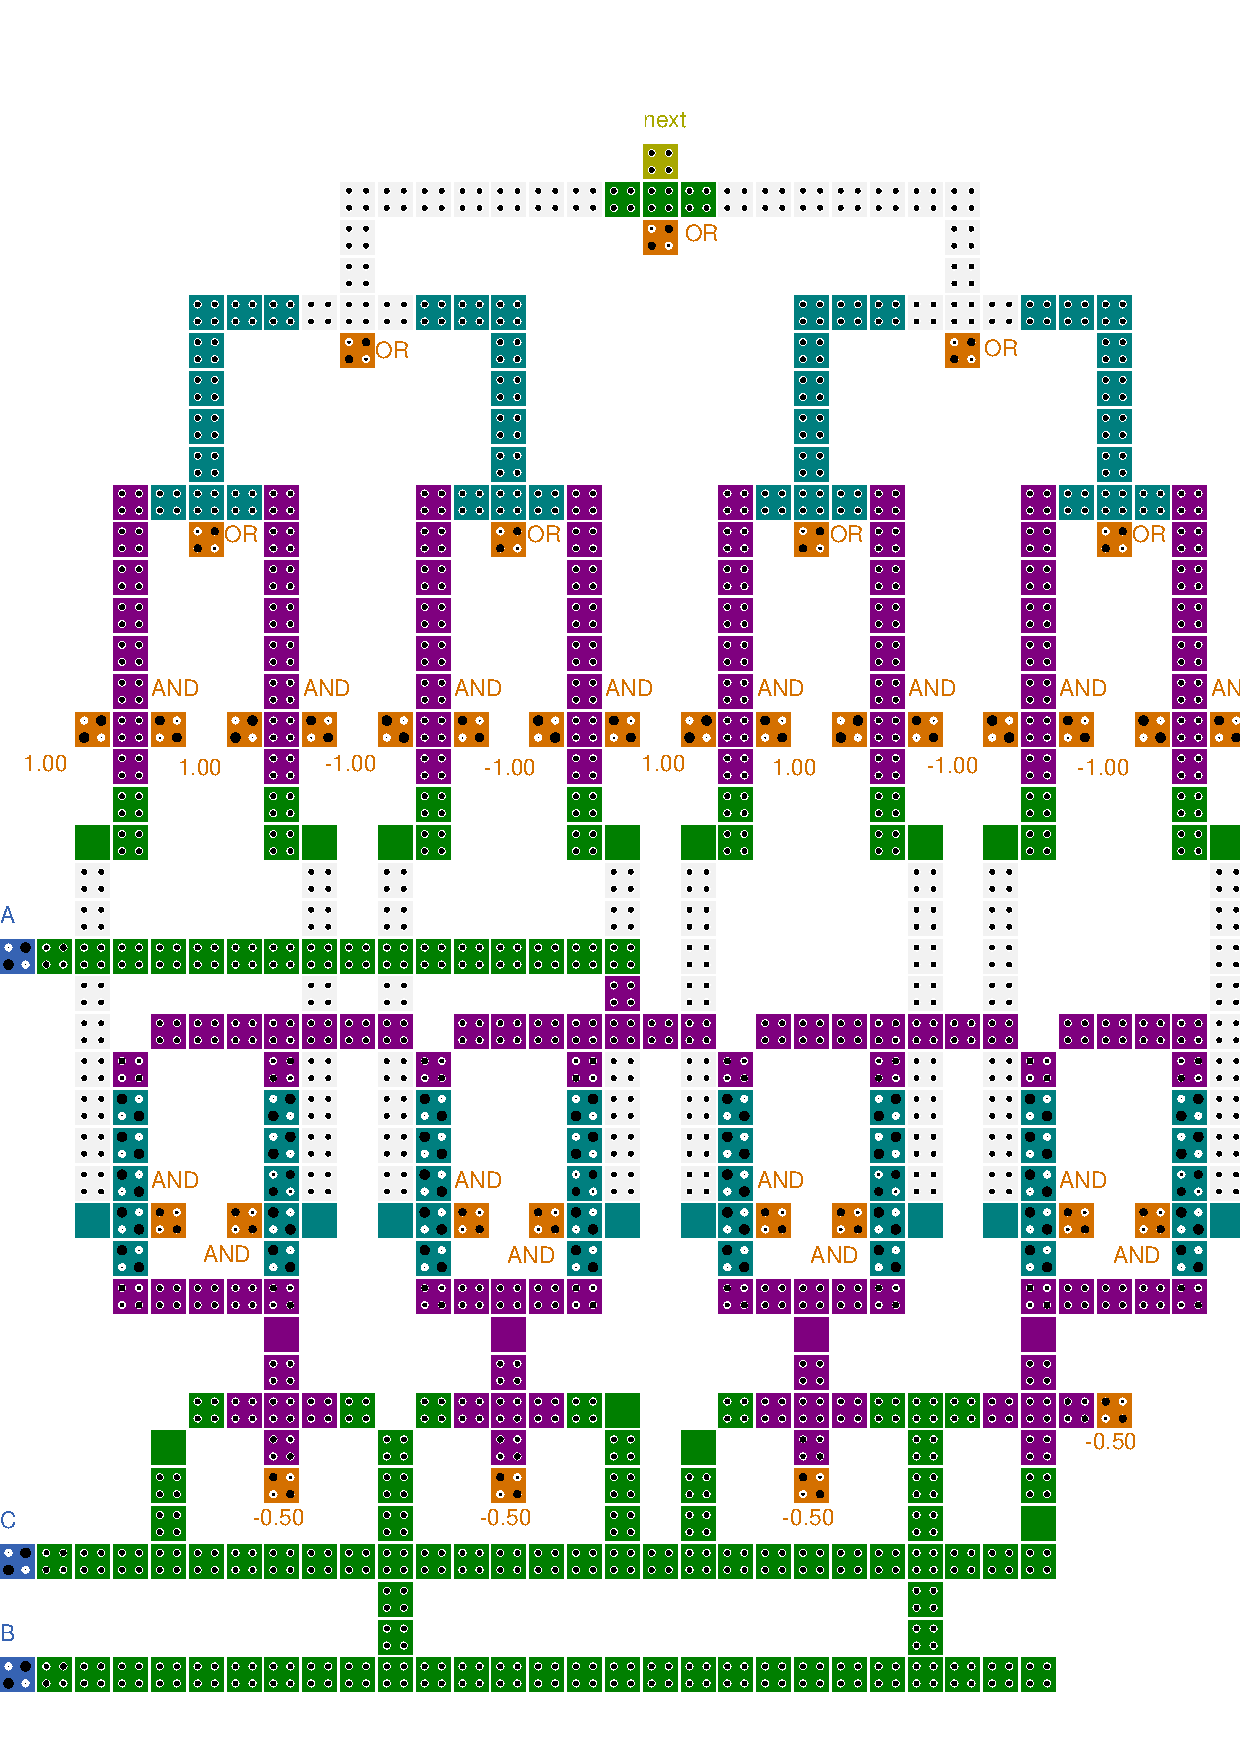
\includegraphics[width=1.0\textwidth]{final}
    \caption{Končna verzija vezja. Bela vodila so postavljena na spodnji sloj.}
    \label{g19:fig:final}
\end{figure}

Končno vezje zaradi preglednosti zavzema relativno veliko prostora, vendar ga je mogoče na večih mestih še optimizirati.
Kot primer bi lahko celotno vezje za izbiro naslednjega stanja postavili direktno pod izhode dekodirnika, brez (belega) vodila, ki povezuje oba dela vezja.
Lahko bi odstranili nekaj celic iz vezja za izbiro naslednjega stanja, saj je trenutno razpotegnjeno.

Končna struktura zavzema površino 33x41 QCA celic in tri sloje, od katerih je eden povezovalni.
Vezje za obdelavo enega vhoda potrebuje dve urini periodi.

\section{Rezultati}
Vezje uspešno implementira 1D celularni avtomat, vendar smo zaradi izboljšanja robustnosti simulacijo izvajali z bistabilno aproksimacijo pri \textbf{100 000 vzorcih} (samples).

Vhode in izhode si lahko interpretiramo tako, da je vhod \textbf{B} trenutno stanje izbrane celice, vhoda \textbf{A} in \textbf{C} pa predstavljata stanji levega in desnega soseda.
Stanja si interpretiramo kot aktivna, če je vrednost signala pozitivna in neaktivna, če je vrednost signala negativna.
Stanje na izhodu \textbf{next} nam pove stanje celice v naslednji iteraciji.

Na Sliki \ref{g19:fig:final_simulation_results} je prikazan celoten izhod simulacije za pravilo \textbf{11001100}.
Za potrditev delovanja smo testirali nekaj pravil, ki so prikazana na Slikah \ref{g19:fig:11110000}, \ref{g19:fig:00110011} in \ref{g19:fig:01010101}.
Ker se za procesiranje porabita 2 urini periodi, je izhod zamaknjen za 2 mesti.

\begin{figure}[H]
    \centering
    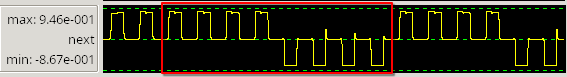
\includegraphics[width=1\linewidth]{11110000.png}
    \caption{Rezultat za pravilo \textbf{11110000}.}
    \label{g19:fig:11110000}
\end{figure}

\begin{figure}[H]
    \centering
    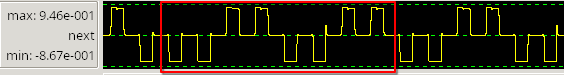
\includegraphics[width=1\linewidth]{00110011.png}
    \caption{Rezultat za pravilo \textbf{00110011}.}
    \label{g19:fig:00110011}
\end{figure}

\begin{figure}[H]
    \centering
    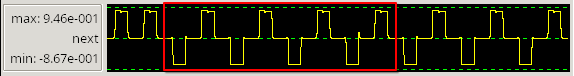
\includegraphics[width=1\linewidth]{01010101.png}
    \caption{Rezultat za pravilo \textbf{01010101}.}
    \label{g19:fig:01010101}
\end{figure}

\begin{figure}[H]
    \sidecaption
    \includegraphics[width=1.0\textwidth]{1d_automata.pdf}
    \caption{Rezultati simulacije vezja v QCA.}
    \label{g19:fig:final_simulation_results}
\end{figure}


\newpage
\section{Zaključek}

Implementirali smo enodimenzionalni celularni avtomat z uporabo tehnologije QCA.
Osnovan je na implementaciji 3-8 dekodirnika \cite{3_8decoder_2}, ki smo jo prilagodili ter ji dodali dodatna vrata za procesiranje izhodov.
IN in ALI vrata smo v QCADesigner-ju implementirali s pomočjo majoritetnih vrat, povezanih na konstante.

Za implementacijo smo uporabili \textbf{541} celic, ki zavzemajo površino 33x41 in so razporejene v 3 sloje.
Naša implementacija uspešno simulira 1D celularni avtomat, ki v dveh urinih periodah sprocesira izhod za naslednjo iteracijo avtomata.

\subsection{Doprionos avtorjev}

Vsi avtorji so prispevali enak delež k projektu.

\appendix